\documentclass{article}
%%%%%%%%%%%%%%%%%%%%%%%%%%%%%%%%%%%%%%%%%%%%%%%%%%%%%%%

%%%%%%%%%%%%%%%%% PACKAGES %%%%%%%%%%%%%%%%%%%%%%%%%%%%
\usepackage{titlepic}
\usepackage{pdfpages}
\usepackage{graphicx}
\usepackage{color,soul}
\usepackage{listings}
\usepackage{color}
\usepackage[capposition=top]{floatrow}
\usepackage{caption}
\usepackage{physics}
\usepackage{amsmath}
\usepackage{hyperref}



%%%%%%%%%%%%%%%%%%%%%%%%%%%%%%%%%%%%%%%%%%%%%%%%%%%%%%
\hypersetup{pdfborder=0 0 0}
\definecolor{codegreen}{rgb}{0,0.6,0}
\definecolor{codegray}{rgb}{0.5,0.5,0.5}
\definecolor{codepurple}{rgb}{0.58,0,0.82}
\definecolor{backcolour}{rgb}{0.95,0.95,0.92}

\lstdefinestyle{mystyle}{
    backgroundcolor=\color{backcolour},   
    commentstyle=\color{codegreen},
    keywordstyle=\color{magenta},
    numberstyle=\tiny\color{codegray},
    stringstyle=\color{codepurple},
    basicstyle=\ttfamily\footnotesize,
    breakatwhitespace=false,         
    breaklines=true,                 
    captionpos=b,                    
    keepspaces=true,                 
    numbers=left,                    
    numbersep=5pt,                  
    showspaces=false,                
    showstringspaces=false,
    showtabs=false,                  
    tabsize=2
}

\lstset{style=mystyle}



%%%%%%%%%%%%%%%%%%%%%%%%%%%%%%%%%%%%%%%%%%%%%%%%%%%%%%

\begin{document}

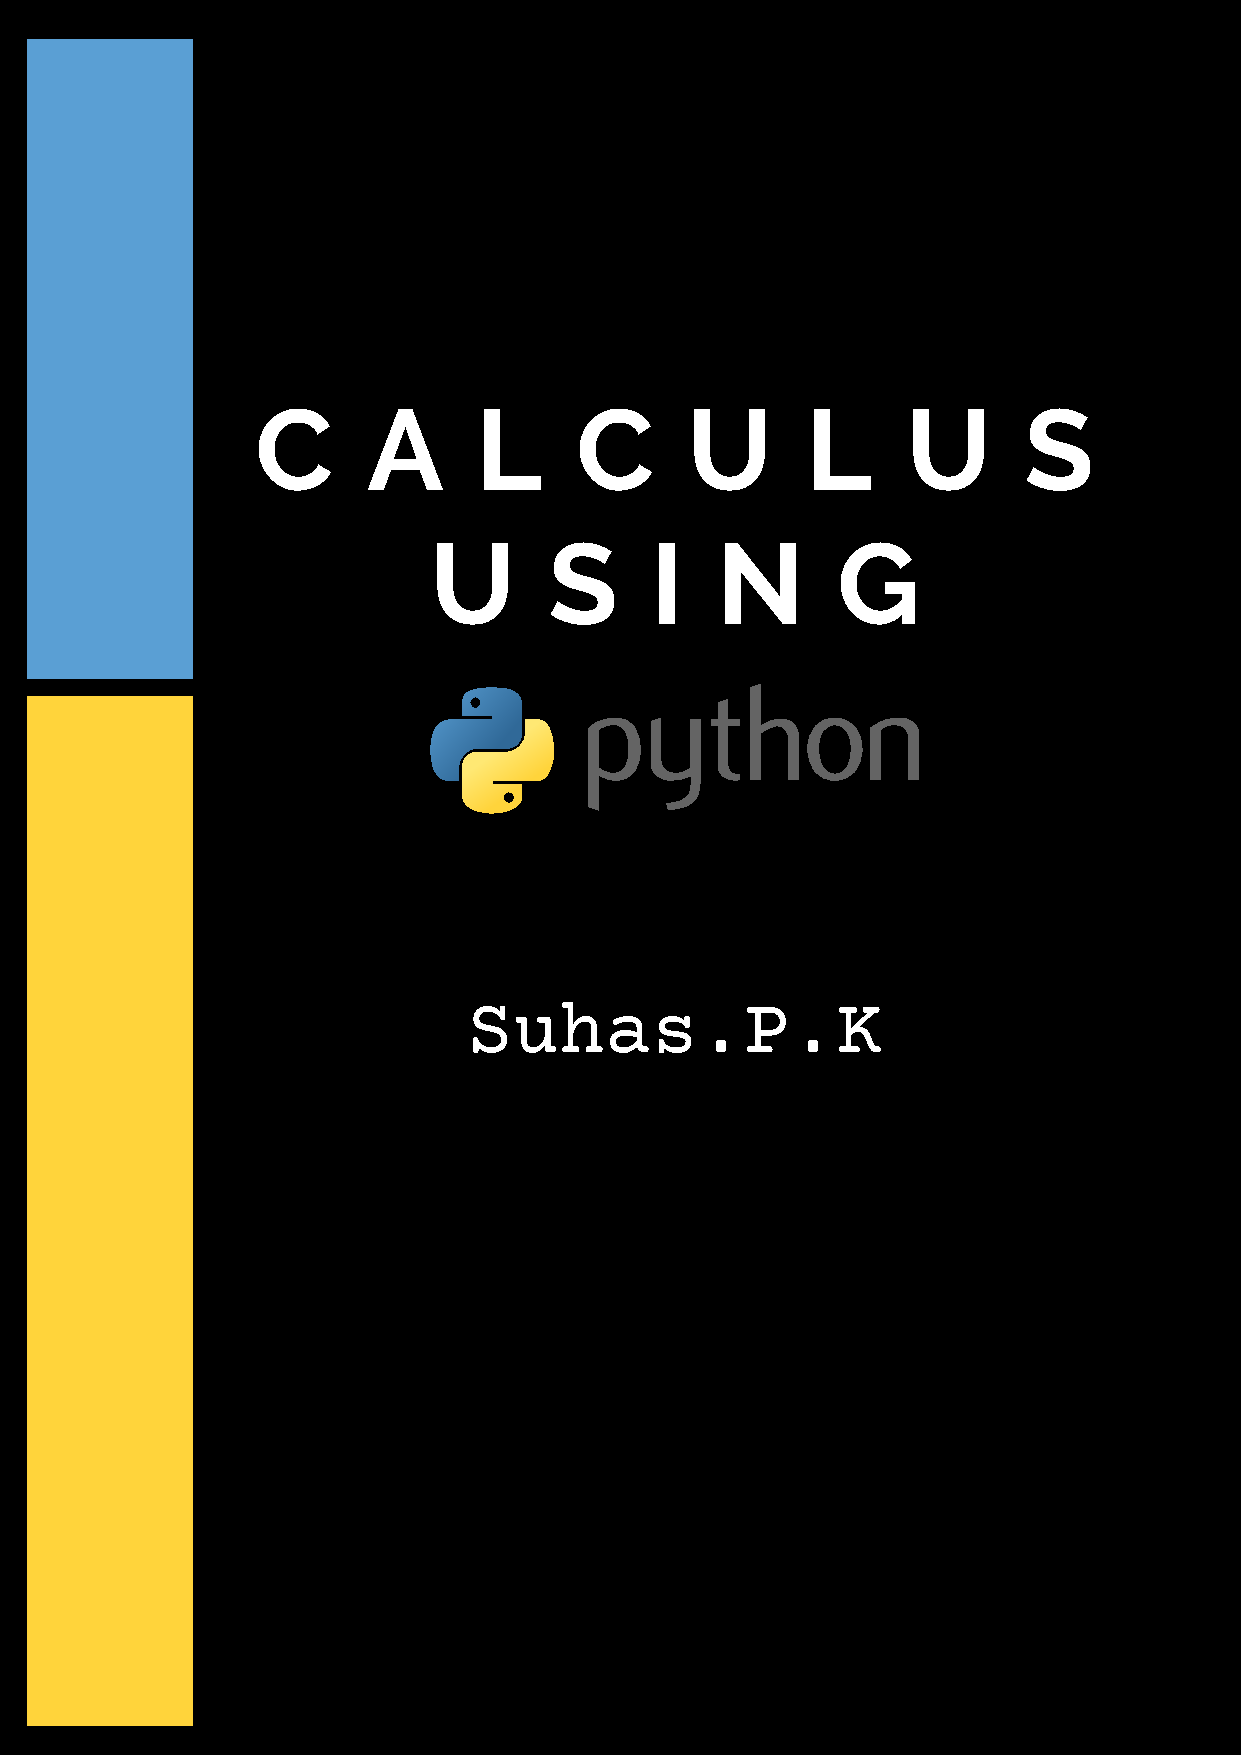
\includepdf[page=1,fitpaper]{1py}


\begin{Large}
\tableofcontents
\end{Large}


\newpage
\section{Limit of a function}
The Python program for this section:
\lstinputlisting[language=Python]
{1_limits.py}

\newpage
\section{Piecewise Function-1}
The Python program for this section:
\lstinputlisting[language=Python]
{piecewise_function.py}
\section{Piecewise Function-2}
The Python program for this section:
\lstinputlisting[language=Python]
{pieceWise_function2.py}

\newpage
\section{Derivative of a polynomial using Symplot}
The Python program for this section:
\lstinputlisting[language=Python]
{poly_diff.py}
\newpage
\section{Derivative of a polynomial using Matplotlib}
The Python program for this section:
\lstinputlisting[language=Python]
{poly_diff1.py}

\newpage
\section{Derivative of a trigonometric function\\ using Symplot}
The Python program for this section:
\lstinputlisting[language=Python]
{trig_diff.py}
\newpage
\section{Derivative of a trigonometric function\\ using Matplotlib}
The Python program for this section:
\lstinputlisting[language=Python]
{trig_diff1.py}
\newpage
\subsection{Exercise-1}
Plot the functions \hl{$f(x) = sin(x+cos(x) + a$} and also it's derivatives for \hl{$a=1,2,3,4$}. 
\\ 
The Python program for this section:
\lstinputlisting[language=Python]
{trig_diff2.py}

\newpage
\section{Tangent Line for the given point.}
The Python program for this section:
\lstinputlisting[language=Python]
{tangentline.py}

\newpage
\section{Critical points of a function.}
\subsection{To find the critical points of a function\\ using empirical method.}
The Python program for this section:
\lstinputlisting[language=Python]
{critical1.py}

\newpage
\subsection{To find the critical points of a function\\ using symbolic method.}
Verify the critical points from the above subsection.
\newline
The Python program for this section:
\lstinputlisting[language=Python]
{critical2.py}

\newpage
\section{Partial derivative }
The Python program for this section:
\lstinputlisting[language=Python]
{part_der.py}

\newpage
\section{Integration}
\subsection{Integration of a polynomial.}
The Python program for this section:
\lstinputlisting[language=Python]
{integrate.py}
\newpage
\subsection{Integration of a trigonometric function.}
The Python program for this section:
\lstinputlisting[language=Python]
{integrate1.py}
\newpage
\subsection{Definite Integration.}
The Python program for this section:
\lstinputlisting[language=Python]
{integrate2.py}

\newpage
\subsection{Trapezoidal Method.}
The Python program for this section:
\lstinputlisting[language=Python]
{trapezoidal(copy).py}

\newpage
\subsection{Simpson's $\frac{1}{3}$ Method.}
The Python program for this section:
\lstinputlisting[language=Python]
{simpson13(copy).py}

\newpage
\section{The Fundamental Theorem of Calculus.}
\begin{equation}
\int \frac{d f(x)}{dx} dx = \frac{d}{dx}\int f(x)dx
\end{equation}
The Python program for this section:
\lstinputlisting[language=Python]
{theorem.py}

\newpage
\section{Area under two curves.}
For given functions $f(x)=x^{2}$ \& $g(x)=x+2$, the area between the two curves whose boundary conditions are the intersection points when the two curves intersect ($a$ \& $b$) is given by,  
\begin{equation}
\int_{a}^{b}[f(x)-g(x)] dx = Area
\end{equation}
The Python program for this section:
\lstinputlisting[language=Python]
{area1.py}

\newpage
\section{Double integration.}
\subsection{Exercise - 1}
For $f(x,y) = x + y$, the double integration with respect to $dx$ \& $dy$ is given by,
\begin{equation}
I = \int \int (x+y)\hspace{0.3cm} dxdy = \frac{x^{2}y}{2}+\frac{y^{2}x}{2}+C
\end{equation}
The Python program for this section:
\lstinputlisting[language=Python]
{db_integrate.py}
\newpage
\subsection{Exercise - 2}
For $f(x,y) = xy$, the double integration with respect to $dx$ \& $dy$ is given by,
\begin{equation}
I = \int \int xy\hspace{0.3cm} dxdy = \frac{x^{2}y^{2}}{4}+C
\end{equation}
The Python program for this section:
\lstinputlisting[language=Python]
{db_integrate1.py}
\newpage
\subsection{Exercise - 3}
For $f(x,y) = x^{2}\frac{sin(y)}{cos(y)}$, the double integration with respect to $dx$ \& $dy$ is given by,
\begin{equation}
I = \int \int x^{2}\frac{sin(y)}{cos(y)}\hspace{0.1cm} dxdy = -\frac{x^{3}log(cos(y))}{3}+C
\end{equation}
The Python program for this section:
\lstinputlisting[language=Python]
{db_integrate2.py}




























\end{document}